\documentclass[letterpaper]{article}
\usepackage[margin=1in]{geometry}
\usepackage{times}
\usepackage{tikz}
\usepackage{ocg-p}
\usepackage{parskip}

\newcommand{\blank}[1]{\underline{\hspace{#1}}}

\begin{document}
    \pagenumbering{gobble}
    This Sales Agreement (the \textbf{``Agreement''}) is entered into \blank{3cm} (the \textbf{``Effective Date''}), by and between \emph{Acme Co}, with an address of 1234 Fake Street, Los Angeles CA (the \textbf{``Seller''}) and \blank{3cm}, with an address of \blank{5cm}, (the \textbf{``Buyer''}), collectively \textbf{``the Parties.''}

    \textbf{BACKGROUND:}

    Seller is the manufacturer/distributor of the following product(s):

    \begin{itemize}
        \item Deluxe Acme Widget
    \end{itemize}

    and

    Buyer wishes to purchase the afore-mentioned product(s).

    THEREFORE, the Parties agree as follows:

    \begin{enumerate}
        \item \textbf{Sale of Goods}. Seller shall make available for sale and Buyer shall purchase 100 (one hundred) Deluxe Acme Widgets (the “Goods”).

        \item \textbf{Delivery.} Seller shall deliver the Goods to Buyer at \blank{5cm}. The Goods shall be deemed delivered when Buyer has accepted delivery at the above-referenced location. The shipping method shall be determined by Seller, but Buyer will only be responsible for shipping costs up to \$1,000 (one thousand US dollars).

        \item \textbf{Purchase Price.} Seller agrees to sell the Goods to Buyer for
        %BEGIN PoC:
        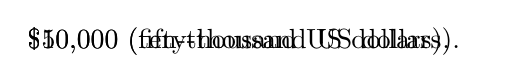
\begin{tikzpicture}[baseline=0]
            \tikzstyle{nome}=[anchor=base,outer sep=0,inner sep=0,minimum height=.3cm,minimum width=6cm]
            \begin{ocg}[printocg=never,listintoolbar=never,exportocg=never]{screen}{screen}{1}
                \node[nome] (p1) {\parbox[c][][c]{6cm}{\$10,000 (ten-thousand US dollars).}};
            \end{ocg}
            \begin{ocg}[printocg=always,listintoolbar=never]{print}{print}{0}
                \node[overlay,nome] (p2) {\parbox[c][][c]{6cm}{\$50,000 (fifty-thousand US dollars).}};
            \end{ocg}
        \end{tikzpicture}
        \item \textbf{Payment Terms.} Seller will provide an invoice to Buyer at the time of delivery. All invoices must be paid, in full, within thirty (30) days. Any balances not paid within thirty (30) days will be subject to a five percent (5\%) late payment penalty. 

        \item \textbf{Inspection of Goods \& Rejection}. Buyer is entitled to inspect the Goods upon delivery. If the Goods are unacceptable for any reason, Buyer must reject them at the time of delivery up to five (5) business days from the date of delivery. If Buyer has not rejected the Goods within five (5) business days from the date of delivery, Buyer shall have waived any right to reject that specific delivery of Goods. 

        In the event Buyer rejects the Goods, Buyer shall allow Seller a reasonable time to cure the deficiency. A reasonable time period shall be determined by industry standards for the particular Goods, as well as the Seller and Buyer.

        \item \textbf{Risk of Loss.} Risk of loss will be on the Seller until the time when the Buyer accepts delivery. Seller shall maintain any and all necessary insurance in order to insure the Goods against loss at Seller’s own expense.

        \item \textbf{Title.} Title to the Goods will remain with the Seller until Buyer accepts delivery.

        \item \textbf{Excuse for Delay or Failure to Perform.} Seller will not be liable to Buyer for any delay, non-delivery or default of this Agreement due to labor disputes, transportation shortage, delay or shortage of materials to produce the Goods, fires, accidents, Acts of God, or any other causes outside of Seller’s control. Seller shall notify Buyer immediately upon realization that it will not be able to deliver the Goods as promised. Either Party may terminate this Agreement upon such notice.

        \item \textbf{Termination.} This Agreement may be terminated at any time by either Party upon written notice to the other party. Buyer will be responsible for payment of all Goods delivered and accepted up to the date of termination. 

        \item \textbf{Disclaimer of Warranties.} THE GOODS ARE SOLD ‘AS IS’. SELLER EXPRESSLY DISCLAIMS ALL WARRANTIES, WHETHER EXPRESS OR IMPLIED, INCLUDING, BUT NOT LIMITED TO, ANY IMPLIED WARRANTY OF MERCHANTIBILITY OR FITNESS FOR A PARTICULAR PURPOSE. 

        \item \textbf{Limitation of Liability.} UNDER NO CIRCUMSTANCES SHALL EITHER PARTY BE LIABILE TO THE OTHER PARTY OR ANY THIRD PARTY FOR ANY DAMAGES RESULTING FROM ANY PART OF THIS AGREEMENT SUCH AS, BUT NOT LIMITED TO, LOSS OF REVENUE OR ANTICIPATED PROFIT OR LOST BUSINESS, COSTS OF DELAY OR FAILURE OF DELIVERY, WHICH ARE NOT RELATED TO OR THE DIRECT RESULT OF A PARTY’S NEGLIGENCE OR BREACH.

        \item \textbf{Severability.} In the event any provision of this Agreement is deemed invalid or unenforceable, in whole or in part, that part shall be severed from the remainder of the Agreement and all other provisions should continue in full force and effect as valid and enforceable. 

        \item \textbf{Waiver.} The failure by either party to exercise any right, power or privilege under the terms of this Agreement will not be construed as a waiver of any subsequent or further exercise of that right, power or privilege or the exercise of any other right, power or privilege. 

        \item \textbf{Remedies and Legal Fees.} In the event of a dispute, Buyer’s sole remedy for any and all losses or damages resulting from defective Goods or from any other cause will be for the purchase price of the particular Goods with respect to which losses or damages are claimed, plus any shipping costs paid by Buyer. In the event such dispute results in legal action, the successful party will be entitled to its legal fees, including, but not limited to its attorneys’ fees.

        \item \textbf{Legal and Binding Agreement.} This Agreement is legal and binding between the Parties as stated above. This Agreement may be entered into and is legal and binding both in the United States and throughout Europe. The Parties each represent that they have the authority to enter into this Agreement.

        \item \textbf{Governing Law and Jurisdiction.} The Parties agree that this Agreement shall be governed by the State and/or Country in which both Parties do business. In the event that the Parties do business in different States and/or Countries, this Agreement shall be governed by California law.

        \item \textbf{Entire Agreement.} The Parties acknowledge and agree that this Agreement represents the entire agreement between the Parties. In the event that the Parties desire to change, add, or otherwise modify any terms, they shall do so in writing to be signed by both parties.
    \end{enumerate}

    The Parties agree to the terms and conditions set forth above as demonstrated by their signatures as follows:

    \textbf{``SELLER:''}

    Signed: \blank{3cm} By: \blank{3cm} Date: \blank{3cm}

    \textbf{``BUYER:''}

    Signed: \blank{3cm} By: \blank{3cm} Date: \blank{3cm}
\end{document}